\documentclass[12pt]{article}

\usepackage[margin=1in]{geometry}
\usepackage{amsmath, amssymb}
\usepackage{enumitem}
\usepackage{booktabs}
\usepackage{graphicx}
\usepackage{float}
\usepackage{longtable}
\usepackage{parskip}
\usepackage{interval}
\usepackage{xcolor}
\usepackage{courier}
\intervalconfig {soft open fences}
\setlength{\parindent}{0pt}

% Colorful hyperlinks within document
\usepackage[colorlinks, citecolor={blue}]{hyperref}

% Verbatim display of R or other code
\usepackage{verbatim, listings}

% More options with captions
\usepackage[format=plain,
labelfont={bf,it},
textfont=it]{caption}

% Figure placement obeys instructions
\usepackage{float}

\title{A multivariate longitudinal model with subject-varying effects for the physical and mental progression of Alzheimer's Disease}
\author{Jesse W.~Birchfield, Robert E. Weiss, and Andrew J. Holbrook}
	
% \begin{figure}[H]
% \centering
% \includegraphics[width=.7\linewidth]{figures/hist\_y0}
% \end{figure}
	
\begin{document}

\maketitle

\pagebreak
\section{Introduction}

Symptoms of Alzheimer's Disease (AD) include both physical and mental decline. Physically, by the prevailing theory {\color{teal}[ref]}, amyloid plaques and neurofibrillary tangles progressively destroy the brain's neurons, beginning in the entorhinal cortex (ERC) and then spreading into the hippocampus and elsewhere {\color{teal}[ref]}. Mentally, subjects begin having difficulty with short-term memory and word recall, and then progressively lose other cognitive and motor abilities {\color{teal}[ref]}. In principle, the mind may be explicable in terms of the nervous system. In practice, it is not, and may never be. For the description of ``objective" biological processes of the brain on one hand, and the description of ``subjective" experiences and behaviors on the other, we have concepts, tools, and measurements that are not only different but incommensurable. A full account of the progression of AD, then, should include both kinds of description. 

Whereas our previous work had the practical aim of improving cortical thickness estimates and enabling earlier detection, the present work is more purely exploratory. We investigate how the effects of the disease co-evolve over time, in relation to the covariates of age, sex, and diagnostic group (disease stage). Using a dataset from the Alzheimer's Diseases Neuroimaging Initiative (ADNI), in particular the ADNI-1 study {\color{teal}[ref]}, we build a multivariate longitudinal model that includes both physical and mental outcomes for each subject at each timepoint. As a physical outcome, we use the thickness of the entorhinal cortex, as estimated by one or more imaging techniques. As a mental outcome, we use the measure taken by ADNI, performance on the Mini Mental State Examination (MMSE) {\color{teal}[ref]}. Our model features hierarchical structure, as varying slopes and intercepts for each subject and outcome (we prefer this term to ``random effects"), with the means and full unstructured covariance matrix of these effects as hyperparameters. This construction enables maximal information sharing across outcomes and subjects, and it allows inference the mean and variance of any of the varying parameters, and the covariance between any subset of them. We discuss all of this in more depth below.

Immediately, we face an array of challenges. First is the challenge of imaging. For brain measurements, we start with magnetic resonance images (MRI), then use different computational ``pipelines" to assemble them into a three-dimensional images, ``segment" them into distinct tissue types, ``label" them as different structures, then estimate their volume and thickness. Although sophisticated, these imaging pipelines are still subject to measurement error. Between pipelines, we see different estimates from the same scan. Within the same pipeline, between scans of the same individual, we see variation beyond that which can explained biologically. The magnitude of measurement error is large enough that it threatens to drown out the subtle effects we hope to detect statistically. And there is no ground truth or gold standard by which to measure the accuracy of these pipelines; we are limited to metrics of internal consistency and predictive power. See our previous work {\color{teal}[ref]} for an attempt to address this issue.

Second is the challenge of psychometrics. Next to the technological marvels of MRI machines and imaging algorithms, a brief questionnaire like the MMSE is very simple and cheap to administer and score. But it is difficult to determine what, exactly, is the construct being measured, or what real entity a score (or score difference) corresponds to, or how accurate the instrument is as an estimator of that construct, or how accurate is an individual instance of measurement. The problem of no ground truth is more pronounced than for the task of imaging, because here it's hard to say even in theory what form ground truth would take. These are interesting and important issues, but beyond the scope of this research. 

Third is the challenge of combining the two measures in a longitudinal model. Brain decay, for a single individual, does not occur uniformly throughout the organ, or at a steady tempo {\color{teal}[ref]}. Across individuals, the spatial and temporal decay patterns vary as well, possibly dependent on factors both measured and unmeasured. We should not expect a simple or consistent pattern of mental decline, either. Even the correlation between physical and mental symptoms is not straightforward. For example, subjects may silently experience several years of brain damage before manifesting any cognitive impairment {\color{teal}[ref]}, and subjects with similar levels of brain damage may perform very differently on cognitive assessments {\color{teal}[ref]}. We propose a model flexible enough to capture this complexity and heterogeneity across outcomes, across time, and across subjects. 

Our different outcomes also have very different numerical properties. Consistent with the hypothesis that they are generated as the true value plus a possible constant bias plus a random measurement error, ERC thickness estimates are positive real numbers with a ``smooth", unimodal, symmetric distribution. A Gaussian fits easily. As questionnaire scores, however, MMSE values are integers, thus discrete and ``coarse"; bounded, on a scale of 0 to 30; and with a very pronounced mode at the right boundary (30) and a long left tail. A Gaussian could hardly do worse. Still, the multivariate normal model has such clear advantages that we would like to adapt our data to the model, rather than the other way around. We propose a transformation of the MMSE data to make this possible. 

We don't just specify a single model \textit{a priori}. After some experimentation with model structure, we build eight models of the chosen class, with different configurations of ERC pipeline and MMSE transformation. We compare their predictive power with Bayesian 5-fold cross-validation. Since the models have different numbers of observations and outcomes on different scales, it takes some ingenuity to devise a metric comparable across all the models. Methodologically, this constitutes a novel combination of techniques and perhaps the most innovative aspect of this project. 

{\color{teal} [Interpretation: what do we learn from the model?]}

\pagebreak
\section{Data}

Our data comes from the Alzheimer's Disease Neuroimaging Initiative (Jack Jr et al., 2008; Petersen et al., 2010; Mueller et al., 2005), a public-private partnership sponsored in part by the National Institute on Aging (NIA). Beginning in October 2004, the three-year longitudinal ADNI-1 study followed a cohort of North American patients comprising 200 elderly controls, 400 with mild cognitive impairment (MCI), and 200 with diagnosed Alzheimer's Disease (AD). At each visit, researchers conducted cognitive assessments and structural MRI scans. Our analysis uses data from 663 of the 800 patients tabulated and made publicly available in Tustison et al. (2019), with a total of 2449 visits. We simply omit those visits that had missing MMSE scores.

{\color{teal} [More description of data? Visualizations of data? Perhaps profile plots with FSLong, ANTsSST, MMSE for some randomly chosen subjects.]}

We analyze output from two eCT pipelines. FreeSurfer and Advanced Normalization Tools (ANTs) use different geometrical constructs to stand in for cortical thickness. FreeSurfer is mesh based, using polygonal meshes representing the gray/white matter surfaces and outer cortical surfaces. We use the version of FreeSurfer optimized for longitudinal measurements of the same subject, hereafter FSLong. ANTs is volumetric, using diffeomorphic mappings. We use the version of ANTs optimized for repeated measurements of the same subject, called the ``single subject template", hereafter ANTsSST. 

The MMSE is a screening test for cognitive impairment. It has 10 questions, takes 5 to 10 minutes to administer, and covers space and time orientation, naming familiar objects, repeating back a phrase, recalling a previous question, manipulating letters and/or numbers, and following instructions. Out of 30 possible points, a score of 24 or more indicates normal cognition, 19-23 indicates mild cognitive impairment, and 18 or below indicates moderate or severe impairment. While it can help differentiate different types of dementia, the test itself is not sufficient for diagnosis.

\pagebreak
\section{Methods}

\subsection{Rationale for model design}

{\color{teal}[
Rationale for treating ECT and MMSE as a multivariate outcome, instead of using ECT as a covariate. (?)

Advantages of multivariate normal: allows us to model error covariance in a matrix, which allows ``strong" information sharing. Allows us to find conditional distribution of one (or a subset) of outcomes given the other(s), which allows for comparing models with a different number of outcomes. It's possible to create a normal/ZINB model, which does fit the data more naturally, but it doesn't have the other features we want.

Advantages of subject-varying effects structure, and of hierarchical modeling for these. No hierarchy for ``fixed" effects. What we can learn from intercept mean and sd, slope mean and sd, correlation of intercept and slope for same outcome, correlation of intercepts for different outcomes, correlations of slopes for different outcomes. All covariance matrices unstructured for max flexibility. 

Modeling of three diagnostic groups completely separately: no overlap in parameters.

No interaction terms.
]}

\pagebreak
\subsection{MMSE transformation}

The 2449 observations of MMSE look like this. Clearly, they do not satisfy the normality assumption, and a multivariate normal model will give poor results.

\begin{figure}[H]
\centering
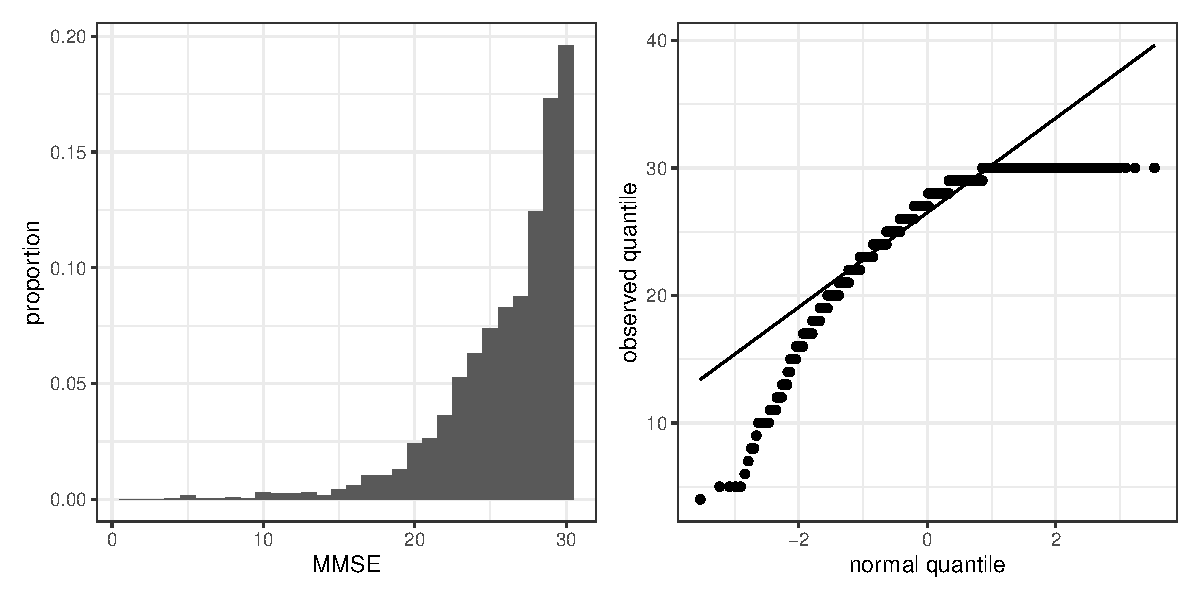
\includegraphics[width=\linewidth]{figures/mmse_before}
\caption{Left: a relative frequency histogram of raw MMSE score for all subjects. It is discrete (integer-valued), bounded (0 to 30), and left-skewed, with a strong mode at the right endpoint. All of these features make it difficult to model with a Gaussian distribution. Right: a normal qq-plot for MMSE. It shows a very poor fit.}
\end{figure}

A Gaussian distribution describes a continuous quantity, not a discrete one. MMSE score is literally a count variable--the number of questions answered correctly on the questionnaire. But since the MMSE's objective is to somehow quantify cognitive capacity, which can reasonably be thought of as continuous, we can treat MMSE score as a ``coarse" or rounded measurement of a continuous latent variable. 

Our first transformation is to consider ``MMSE loss"--questions missed--rather than MMSE, by subtracting the raw value from 30. So a score of 30 becomes 0, a score of 29 becomes 1, and so on. We also imagine a kind of threshold, where cognitive decline has to reach a certain point before the subject would miss another question, so the MMSE loss represents a rounding \textit{down} of the latent quantity. This justifies the step of adding $0.5$ to each value. So define $y = 30 - MMSE + 0.5$. 

Our next step is much easier with a single-parameter probability distribution, and this looks like a histogram of a sample from some Exponential distribution. We assume $F(y) = 1 - e^{-\lambda y}$. The maximum likelihood estimate of $\lambda$ is the maximum value of the polynomial $\Pi_{i=1}^{n}\left[ e^{-\lambda y_i} - e^{-\lambda (y_i + 1)} \right]$, which R easily computes as $\hat{\lambda} = 0.236$. 

The probability integral transform states that if random variable $W$ has continuous monotonic CDF $F$, then random variable $F(W)$ has a $Unif(0,1)$ distribution. Conversely, if $U \sim Unif(0,1)$, and $G$ is the continuous monotonic CDF of random variable $X$, then random variable $G^{-1}(U)$ has the same distribution as $X$. Letting $F$ in the theorem be the exponential CDF with parameter $\hat{\lambda}$, and letting $G$ be the standard normal CDF $\Phi$, the transformation $\Phi^{-1}(F(Y))$ will have standard normal distribution, at least to the extent that $F$ describes the distribution of $Y$. 

\begin{figure}[H]
\centering
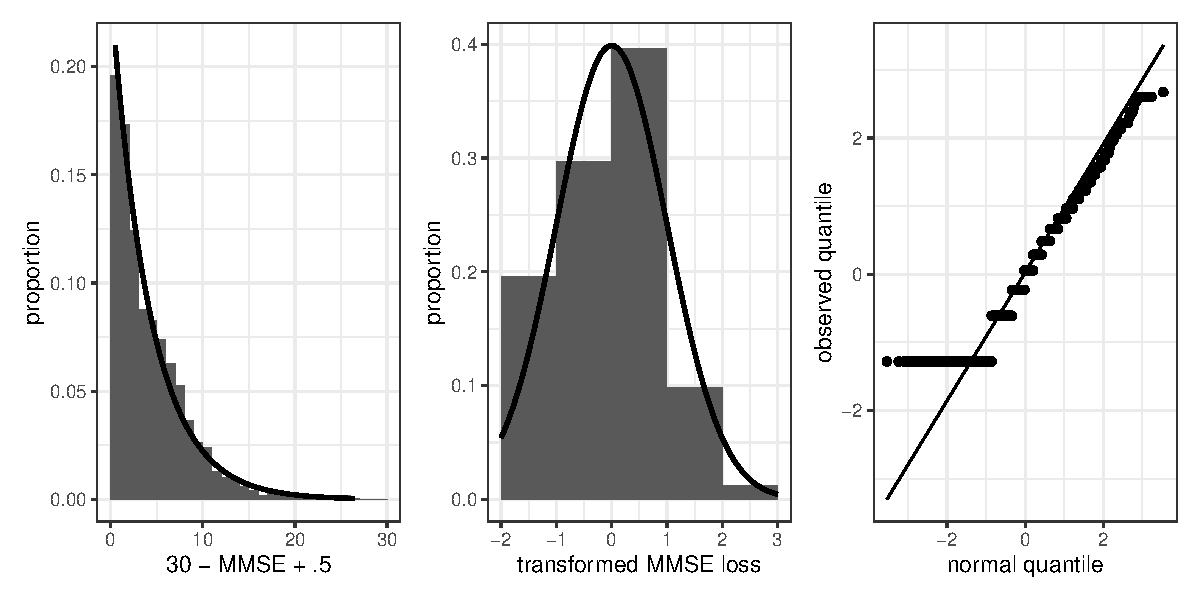
\includegraphics[width=\linewidth]{figures/mmse_after}
\caption{Left: Histogram of MMSE loss, defined as $30 - MMSE + .5$, overlaid with an Expo(.236) density, the best-fitting Exponential model by maximum likelihood. The histogram looks like a plausible sample from this density. Center: a histogram of MMSE transformed according to $h(y) = \Phi^{-1}(1 - e^{-.236(30-y+.5)})$, overlaid with a N(0,1) density. While not a perfect fit, it is a substantial improvement on the original. Right: a normal qq-plot of transformed MMSE loss. The main departure from normality occurs because of the high number of perfect MMSE scores.}
\end{figure}

It's true that this technique will give $Y$ a \textit{marginally} normal distribution, whereas the assumption of the multivariate normal regression model is that $Y$ is \textit{conditionally} normal given the predictors. But this is does not make much of a difference in practice. If $Y|X \sim N(X\beta, \sigma_{Y}^{2})$, and $X \sim N(\mu_X, \sigma_{X}^{2})$, then $Y \sim N(\mu_X, \sigma_{X}^{2} + \sigma_{Y}^{2})$; it is still normal. If $X$ is binary or discrete, then $Y$ is a mixture of normals; when the differences between the means of the mixture components are small compared to the overall variance, the mixture distribution is empirically not much different from a true normal distribution with the same mean and variance. 

\pagebreak
\subsection{Model specification}

Here we describe the model in prose, and afterward we formally specify it in symbols. For each subject, and at each timepoint, we have a bivariate or trivariate outcome, consisting of (i) ERC, as estimated by FSLong, ANTsSST, the arithmetic mean of the two, or both, and (ii) MMSE loss, either untransformed or transformed. We model these as bivariate or trivariate normal, where the mean is a linear function of predictors described shortly, and the error covariance matrix is unstructured, to be estimated from the data. Predictors are age at baseline, centered by subtracting the mean age at baseline across all 663 subjects, a gender indicator, and time of visit in years since baseline. For each outcome, we have a separate set of coefficients. The coefficients for age and gender are ``fixed", in the sense that they do not vary by subject and do not have hyperparameters. The intercepts and slopes of the outcomes \textit{do} vary by subject, and we consider them as draws from an underlying multivariate normal distribution with a common mean and an unstructured covariance matrix. This hierarchical structure allows for information sharing across outcomes, across timepoints, and across subjects. We do not add any additional covariance across timepoints other than that induced by the slopes. Finally, for each diagnostic group--CN, MCI, AD--we fit a completely separate set of coefficients and hyperparameters, so that we effectively have three separate regressions. 

Formally, let $i$ index subjects, $i=1,...,N$. For our data, $N=663$. Let $j$ index timepoints, $j=1,...,J_i$. For our data, $J_i$ is between 2 and 6 for all $i$. Let $k$ index outcomes, $k=1,...,K$. For models 1-3 and 4-6, $K=2.$ For models 4 and 8, $K=3$. Let $\ell$ index groups, $\ell=1,...,L$. For our data, $\ell=1,2,3$ for CN, MCI, AD respectively. Let $m$ index covariates or coefficients. So we have five sets of indices $i,j,k,\ell,m$, not all of which are relevant for any given quantity. To avoid confusion, we use dots as placeholders for irrelevant indices, so that $x_{7...2}$ is covariate $m=2$ for subject $i=7$, which is the same for all timepoints $j$ and outcomes $k$ and has group $\ell$ determined by $i$. 

Let $\boldsymbol{y_{ij.\ell}}$ be the $K$-vector of observation $ij$, where subject $i$ is in group $\ell$. Let $\boldsymbol{\epsilon_{ij.\ell}}$ be the $K$-vector of errors for observation $ij$, for $i$ in group $\ell$. Both for computation and for interpretability, we factor all covariance matrices into a diagonal matrix of standard deviations and a matrix of correlations, e.g. $\boldsymbol{C=SRS'}$, and we write the standard deviations as a vector. Then, when specifying multivariate normal distributions, we use the notation $N$(mean, sd vector, correlation matrix). Let $\boldsymbol{\sigma_{...\ell}}$ be the $K$-vector of standard deviations for the error vectors $\boldsymbol{\epsilon_{ij.\ell}}$, and let $\boldsymbol{R_{...\ell}}$ be the $K \times K$ correlation matrix.

Let $x_{i...1}$ be baseline age in years, mean-centered, for subject $i$. Let $x_{i...2}$ be the indicator that subject $i$ is male, for subject $i$. Let $\boldsymbol{x_{ij..}'} = \begin{bmatrix}x_{ij..1} & ... & x_{ij..M}\end{bmatrix}.$ Generally, we use $\alpha$ to denote subject-invariant effects and $\beta$ to represent subject-varying effects. Let $\boldsymbol{\alpha_{..k\ell}'}$ be the 2-vector of coefficients for each $\boldsymbol{x_{ij..}'}$ outcome $k$, group $\ell$. Let $t_{ij...}$ be time in years since baseline for subject $i$, timepoint $j$. Let $\boldsymbol{z_{ij...}'} = \begin{bmatrix} 1 & t_{ij..} \end{bmatrix}$. Let $\boldsymbol{\beta_{i.k\ell}}$ be the 2-vector of subject-varying intercept and slope for subject $i$, outcome $k$, group $\ell$. Let $\boldsymbol{\beta_{i..\ell}}$ be the concatenated $2K$-vector $\begin{bmatrix} \boldsymbol{\beta_{i.1\ell}'} & ... & \boldsymbol{\beta_{i.K\ell}'} \end{bmatrix}'$. Let  $\boldsymbol{\mu_{...\ell}}$ be the $2K$-vector of means for the vectors $\boldsymbol{\beta_{i..\ell}}$, let $\boldsymbol{\tau_{...\ell}}$ be the $2K$-vector of standard deviations, and let $\boldsymbol{\Omega_{...\ell}}$ be the $2K \times 2K$ correlation matrix. 

This complexity of notation pays off, because it allows us to express the model quite compactly, as
$$
\boldsymbol{y_{ij.\ell}} = 
\begin{bmatrix}
	\boldsymbol{x_{ij..}'\alpha_{..1\ell} + z_{ij..}'\beta_{i.1\ell}} + \epsilon_{ij1\ell} \\
	\boldsymbol{x_{ij..}'\alpha_{..2\ell} + z_{ij..}'\beta_{i.2\ell}} + \epsilon_{ij2\ell} \\
	\boldsymbol{x_{ij..}'\alpha_{..3\ell} + z_{ij..}'\beta_{i.3\ell}} + \epsilon_{ij3\ell}	
\end{bmatrix}
$$
$$
\boldsymbol{\beta_{i..\ell}} \mid \ \boldsymbol{\mu_{...\ell}}, \boldsymbol{\tau_{...\ell}}, \boldsymbol{\Omega_{...\ell}}
\sim
N_4 \left(\boldsymbol{\mu_{...\ell}}, \boldsymbol{\tau_{...\ell}}, \boldsymbol{\Omega_{...\ell}}\right)  
$$
$$
\boldsymbol{\epsilon_{ij.\ell} \mid \sigma_{...\ell}, R_{...\ell}}
\sim 
N_2 \left(\boldsymbol{0, \sigma_{...\ell}, R_{...\ell}}\right).
$$

We choose our priors to be as uninformative as possible while still allowing decent convergence in posterior sampling. We keep them identical across models and groups, and virtually identical across outcomes and coefficients. All prior distributions are independent of each other unless otherwise stated. Error sd's have prior $Expo(1)$, parameterized by rate. All $\alpha$ parameters have prior $N(0,2)$. For ERC outcomes, means of subject-specific intercepts have prior $N(7,3)$ and sd's have $Expo(1)$, while means of subject-specific slopes have prior $N(0,1)$ and sd's have $Expo(5)$. For MMSE outcomes, means of subject-specific intercepts have prior $N(0,2)$ and sd's have $Expo(1)$, while means of subject-specific slopes have prior $N(0,2)$ and sd's have $Expo(1)$. Finally, all correlation matrices have prior $LKJCorr(1)$. This is the Lewandowski-Kurowicka-Joe distribution, a single-parameter 
family of correlation matrices (Gelman et al., 1995), argued to be superior to the traditional inverse Wishart prior distribution {\color{teal}[ref: Stan manual]}. A prior parameter $\eta=1$ indicates neutrality about whether the correlation is positive, negative, or 0. 

Our eight candidate models have the same structure, differing only in the  outcome variables, as shown in Table 1:

\begin{table}[H]
\centering
\caption{Candidate models}
\begin{tabular}{l|l|l|l}
\toprule
& $y_1$ & $y_2$ & $y_3$\\
\midrule
1 & FSLong & untransformed MMSE \\
2 & ANTsSST & untransformed MMSE \\
3 & ECTavg & untransformed MMSE \\
4 & FSLong & ANTsSST & untransformed MMSE \\
5 & FSLong & transformed MMSE \\
6 & ANTsSST & transformed MMSE \\
7 & ECTavg & transformed MMSE \\
8 & FSLong & ANTsSST & transformed MMSE \\
\bottomrule
\end{tabular}
\end{table}

\pagebreak
\subsection{Computation}

We use the R programming language, supplemented by the package dplyr for all data management, and by the package pracma for advanced mathematical operations. To specify and fit the model, we use Stan, an open-source Bayesian software application, interfacing with R through the rstan package. We include our model scripts as an appendix, and the Stan file and all R scripts and regression results at \url{https://github.com/jwbirchfield/ad\_progression/}. Stan uses Hamiltonian Monte Carlo, a flavor of Markov Chain Monte Carlo to draw samples—each of which is a complete vector of parameters—from the joint posterior distribution. An advanced extension of HMC called the No U-Turn Sampler (NUTS) improves sampling efficiency. As the number of MCMC samples increases, the distribution of MCMC samples converges to the actual joint posterior distribution. Fortunately, the marginal distribution of each parameter in the MCMC samples converges to its actual marginal posterior distribution as well. To fit each of the eight models, we ran 4 chains in parallel with 6000 iterations each, which we thinned by a factor of 3 to get 8000 iterations. Effective sample sizes are all greater than 300, and R-hat statistics are no greater than 1.01. See Appendix A for the Stan code for the model. In the cross-validation stage, for each of the eight models and for each of the 5 folds, we ran 4 chains in parallel with 2000 iterations each, which we thinned by a factor of 2 to get 4000 iterations. We calculated ELPD and other fit statistics from the posterior samples, using custom R scripts.

\pagebreak
\subsection{Model comparison}

\pagebreak
\section{Discussion}

\pagebreak
\section{Appendix A: Stan code}

\begin{verbatim}
// GENERAL SCRIPT FOR 8 MODELS

data{
  
  int<lower=1> I; // number of subjects
  int<lower=1> N; // total number of observations, each n is ij
  array[N] int<lower=1> id; // id of nth observation
  array[I] int<lower=1> group; // diagnostic group of subject i (CN=1, MCI=2, AD=3)
  int<lower=1> K; // number of outcomes
  array[N] vector[K] y; // vector of outcomes (e.g. FSLong, ANTsSST, MMSE_loss) for n = 1:N
  array[N] row_vector[4] X; // 1, t, age_c, male
  
}

transformed data {}

parameters{
  
  array[3] vector[2*K] alpha;
  array[3] vector[2*K] mu_beta; 
  array[3] vector<lower=0>[2*K] sigma_beta; 
  array[3] vector<lower=0>[K] sigma_epsilon; 
  array[3] cholesky_factor_corr[2*K] L_Rho_beta; 
  array[3] cholesky_factor_corr[K] L_Rho_epsilon; 
  array[I] vector[2*K] z;

}

transformed parameters{
  
  array[N] vector[K] mu_y; 
  array[I] vector[2*K] beta; 
  array[3] cholesky_factor_cov[2*K] L_Sigma_beta;
  array[3] cholesky_factor_cov[K] L_Sigma_epsilon; 

  
  for(l in 1:3){
    L_Sigma_epsilon[l] = diag_pre_multiply(sigma_epsilon[l], L_Rho_epsilon[l]);
    L_Sigma_beta[l] = diag_pre_multiply(sigma_beta[l], L_Rho_beta[l]);    
  }
  
  for(i in 1:I){
    // equiv to beta[i] ~ multi_normal(mu_beta[group[i]], Sigma_beta[group[i]])
    beta[i] = mu_beta[group[i]] + L_Sigma_beta[group[i]] * z[i];
  }

  if(K == 2){
    for(n in 1:N){
      mu_y[n] = [ X[n] * append_row(beta[id[n]][1:2], alpha[group[id[n]]][1:2]),
                  X[n] * append_row(beta[id[n]][3:4], alpha[group[id[n]]][3:4])]';
    }
  }

  if(K == 3){
    for(n in 1:N){
      mu_y[n] = [ X[n] * append_row(beta[id[n]][1:2], alpha[group[id[n]]][1:2]),
                  X[n] * append_row(beta[id[n]][3:4], alpha[group[id[n]]][3:4]),
                  X[n] * append_row(beta[id[n]][5:6], alpha[group[id[n]]][5:6]) ]';
    }
  }
  
}

model{

// Likelihood

  for(n in 1:N){
    y[n] ~ multi_normal_cholesky(mu_y[n], L_Sigma_epsilon[group[id[n]]]);
  }

  // Priors
  for(l in 1:3){
    
    alpha[l] ~ normal(0,2); 
    mu_beta[l][1] ~ normal(7,3); // y1 intercept mean
    mu_beta[l][2] ~ normal(0,1); // y1 slope mean
    sigma_beta[l][1] ~ exponential(1); // y1 intercept sd
    sigma_beta[l][2] ~ exponential(5); // y1 slope sd
    
    if(K == 2){
      mu_beta[l][3] ~ normal(0,2); // MMSE intercept mean
      mu_beta[l][4] ~ normal(0,2); // MMSE slope mean
      sigma_beta[l][3] ~ exponential(1); // MMSE intercept sd
      sigma_beta[l][4] ~ exponential(1); // MMSE slope sd
    }
    
    if(K == 3){
      mu_beta[l][3] ~ normal(7,3); // y2 intercept mean
      mu_beta[l][4] ~ normal(0,1); // y2 slope mean
      mu_beta[l][5] ~ normal(0,2); // MMSE intercept mean
      mu_beta[l][6] ~ normal(0,2); // MMSE slope mean
      sigma_beta[l][3] ~ exponential(1); // y2 intercept sd
      sigma_beta[l][4] ~ exponential(5); // y2 slope sd  
      sigma_beta[l][5] ~ exponential(1); // MMSE intercept sd
      sigma_beta[l][6] ~ exponential(1); // MMSE slope sd
    }
    
    L_Rho_beta[l] ~ lkj_corr_cholesky(1);
    sigma_epsilon[l] ~ exponential(1);
    L_Rho_epsilon[l] ~ lkj_corr_cholesky(1);
    
  }
  
  // random effects distribution
  for(i in 1:I){
    z[i] ~ std_normal();
  }
  
}

generated quantities {

  vector[N] log_lik;
  array[3] matrix[2*K,2*K] Rho_beta;
  array[3] matrix[K,K] Rho_epsilon;

  for(n in 1:N){
    log_lik[n] = multi_normal_cholesky_lpdf(y[n] | mu_y[n], L_Sigma_epsilon[group[id[n]]]);
  }

  for(l in 1:3){
    Rho_beta[l] = L_Rho_beta[l] * L_Rho_beta[l]';
    Rho_epsilon[l] = L_Rho_epsilon[l] * L_Rho_epsilon[l]';  
  }

}
\end{verbatim}

\end{document}



\section{Data description}

Problems with using one response as a time-varying covariate (Weiss 2005): We cannot use observations with one response or the other but not both: reduced sample size, dropping not at random can cause bias. Which response should be treated as the response and which should be treated as the covariate? Results may be different. Whichever response is being used as a predictor may be affected by the other covariates in the analysis. 

\section{Variable transformation} 

\section{Model design}

\subsection{Notation}

\subsection{Specification}

\subsection{Rationale, justification}

Features and advantages of hierarchical random effects model. Why did we make the modeling choices we did? Why are our priors reasonable?

\section{Computation}

Getting this model to converge in Stan is challenging. Maybe include an appendix for how I achieve this.

\section{Model comparison}

\subsection{Method}

We have four models with untransformed MMSE, four with transformed MMSE. 

How do we compare these 8 models on a commensurable scale? Cross-validation is the gold standard for model comparison. We use 5-fold Bayesian CV on the LEPD (log expected predictive density, to be defined). Since some models are bivariate and some are trivariate, we find the CV LEPD of MMSE conditional on the other outcome(s). Since some models use untransformed MMSE and some use transformed MMSE, we apply the Jacobian correction. Putting these techniques together is complicated; this may be the first time this particular combination of techniques has been used. 
[Section on methodological details]

We also integrate out the random effects beta and do it again. [Why?] 

\subsection{Results}

The best model by conditional LEPD is the one with outcomes (ANTsSST, transformed MMSE). [Maybe run longer CV chains to make sure.]

The best model by marginal conditional LEPD is the one with outcomes (FSLong, transformed MMSE). 

Effect of transformation: Comparing models with transformation to the corresponding models without, we see LEPD increase by about 700. Since there are 2449 observations in the data, and exp(700/2449)=1.33, the transformed model has a typical likelihood 1.33 times higher per observation. (How else to interpret this? Likelihood ratio? Bayes factor?)

\section{Analysis}

Make inferences from the best model.

\section{Discussion}

What is noteworthy, from clinical side or statistical side? Where do we go next?

***

Earlier work (and probably other people's work) treated MMSE as dependent on ERC. This is scientifically reasonable, but we can do without this assumption, treat the two as coevolving, correlated outcomes

ANTs, FS
The best FS is FSLong, designed specifically for longitudinal data
The best ANTs for this is ANTsSST